\documentclass[journal,onecolumn]{IEEEtran}
\usepackage{amsmath,amssymb}
\usepackage{graphicx}
\usepackage{booktabs}
\usepackage[utf8]{inputenc}
\graphicspath{{figs/}}
\setlength{\emergencystretch}{8em}
\begin{document}

\title{Supplementary Material for ``When Does Drift Gating Pay Off? A
Reproducible Measurement Study of Drift-Aware Page Replacement''}
\author{M. Qasim, H. Tahir, H. Ahmad, and M. G. Ghouri}
\maketitle

\section{S1.\ Exact commands}

All commands are run from \texttt{reproduction/}. The authoritative simulator
source is \texttt{sim\_full.cpp}; \texttt{sim\_full\_diag.cpp} and
\texttt{sim\_full\_bench.cpp} are additive diagnostic and timing-only builds.

\subsection{S1.1 Primary study}
\begin{verbatim}
g++ -O2 -std=c++17 -o sim_full sim_full.cpp
python3 sweep_selection.py --jobs 4
./sim_full --seed 100 --stable-per-prim 3 --per-scenario 8 \
  --ncand 5 --kfrac 0 --z 1.28 --edelay 10 \
  --out main_study_training.csv --det main_study_training_detection.csv
./sim_full --seed 5001 --ncand 5 --kfrac 0 --z 1.28 --edelay 10 --ablations \
  --out main_study_results.csv --det main_study_detection.csv
\end{verbatim}

\subsection{S1.2 Boundary offsets (Table IX)}
\begin{verbatim}
for off in 250 500 1000 1370; do
  ./sim_full --seed 5001 --ncand 5 --kfrac 0 --z 1.28 --edelay 10 \
    --da-only --phase-offset $off \
    --out results_offset${off}.csv --det detection_offset${off}.csv
done
python3 generate_offset_table.py
\end{verbatim}
Offset 0 is \texttt{main\_study\_detection.csv}. The script reads all five
CSVs and writes \texttt{latex/offset\_table.tex}.

\subsection{S1.3 Public FIU traces}
\begin{verbatim}
python3 convert_public_traces.py --all --limit 1000000
./sim_full --np 1048576 --C 20000 --warm 100000 \
  --ncand 5 --kfrac 0 --z 1.28 --edelay 10 \
  --s3frac 0.05 --twoqkin 125 --lprthr 0.1 \
  --lecarlr 0.6 --lirsfrac 0.05 \
  --methods LRU,FIFO,2Q,ARC,S3-FIFO,DA,ContShadow,OPT \
  --trace fiu_homes-110108-112108.oracleGeneral.bin \
  --trace fiu_ikki-110108-112108.oracleGeneral.bin \
  --trace fiu_madmax-110108-112108.oracleGeneral.bin \
  --trace fiu_online.cs.fiu.edu-110108-113008.oracleGeneral.bin \
  --trace fiu_webmail.cs.fiu.edu-110108-113008.oracleGeneral.bin \
  --trace fiu_webresearch-030409-033109.oracleGeneral.bin \
  --out public_trace_results.csv --det public_trace_detection.csv
\end{verbatim}

\subsection{S1.4 Public-trace diagnostics}
\begin{verbatim}
g++ -O2 -std=c++17 -o sim_full_diag sim_full_diag.cpp
./sim_full_diag --np 1048576 --C 20000 --warm 100000 --ncand 5 \
  --kfrac 0 --z 1.28 --edelay 10 --s3frac 0.05 --twoqkin 125 \
  --lprthr 0.1 --lecarlr 0.6 --lirsfrac 0.05 \
  --methods LRU,S3-FIFO,DA,ContShadow \
  --detail-log public_detail.csv \
  --out public_diag_results.csv --det public_diag_detection.csv \
  --trace <the six fiu_*.bin files above>
\end{verbatim}
The diagnostic build is behaviourally identical to the released simulator:
0 mismatches in \texttt{scenario, seed, method, miss\_ratio, switches,
shadow\_evals} over the 110-trace main study, and byte-identical detection CSVs.

\subsection{S1.5 Public-trace parameter re-selection}
\begin{verbatim}
python3 split_public_traces.py          # 500k train / held-out suffix
python3 sweep_public_selection.py       # 48 configs on six prefixes
sh run_public_reselect.sh               # frozen vs re-selected on suffixes
\end{verbatim}

\subsection{S1.6 Cost model and direct evaluation timing}
\begin{verbatim}
python3 cost_model.py
python3 bootstrap_cost_model.py
g++ -O2 -std=c++17 -o sim_full_bench sim_full_bench.cpp
./sim_full_bench --seed 5001 --ncand 5 --kfrac 0 --z 1.28 --edelay 10 \
  --da-only --out bench_main.csv --det bench_main_det.csv
\end{verbatim}

\section{S2.\ Raw CSV rows removed from the body}

\subsection{S2.1 Detection schema}
The nine columns of every detection CSV are: scenario, seed, method, number of
true boundaries, detected boundaries, detection delays (semicolon-separated),
spurious confirmations, total confirmations, and false confirmations after
reference 100,000.

\subsection{S2.2 Offset 0 and 1{,}370 first rows per scenario}
\begin{verbatim}
stable,5001,DA,0,0,,1,1,0
abrupt,6001,DA,5,5,2000;2000;4000;2000;2000;,1,6,0
gradual,7001,DA,5,1,0;,5,6,0
recurring,8001,DA,5,5,4000;2000;4000;2000;4000;,1,6,0
composite,9001,DA,4,3,2000;2000;2000;,2,5,0
\end{verbatim}
\begin{verbatim}
stable,5001,DA,0,0,,1,1,0
abrupt,6001,DA,5,5,630;630;2630;630;2630;,1,6,0
gradual,7001,DA,5,1,630;,5,6,0
recurring,8001,DA,5,5,2630;630;2630;630;2630;,1,6,0
composite,9001,DA,4,3,630;630;630;,2,5,0
\end{verbatim}

\subsection{S2.3 Stable-trace confirmation positions}
The 23 confirmations on stable traces occur at references
18{,}000 ($\times 6$), 28{,}000 ($\times 5$), 30{,}000 ($\times 2$),
34{,}000 ($\times 2$), 36{,}000, 38{,}000, 56{,}000, 68{,}000 ($\times 2$),
72{,}000, 74{,}000 and 160{,}000. Only the last exceeds reference 100{,}000.

\subsection{S2.4 Public-trace per-candidate diagnostics}
\texttt{public\_diagnostic\_summary.csv} records, for each trace, the initial
candidate pick, the first evaluation's miss counts for candidates 0--4
(0 LRU, 1 LFU-A, 2 2Q, 3 MRU, 4 S3-FIFO), the maximum CUSUM statistics, and the
number of confirmed alarms. All six initial picks were candidate 0 and all
five first-evaluation counts were identical.

\section{S3.\ Diagnostic event-log schema}
The \texttt{--detail-log} CSV has columns kind, scenario, seed, method, ep, t,
field, value. Kinds are \texttt{eval} (window size, start epoch, raw block
count and per-candidate miss totals), \texttt{decide} (cost margin, active
candidate, per-candidate margin, lower confidence bound and score, final pick),
\texttt{cusum} (standardised miss deviation and both CUSUM statistics before
and after update), \texttt{alarm} (KS $p$-value, sample size and confirmation
flag), \texttt{wait} (dwell blocks), \texttt{switch} (purge counts) and
\texttt{component} (per-trace activation totals). All logging calls are
no-ops unless \texttt{--detail-log} is supplied.

\section{S2. Literature Review Tables}

\begin{table*}[!t]
\caption{Table S.I. Comparative Summary of the Reviewed Studies and Closest Prior Art}
\label{tab:lit}
\small
\begin{tabular}{@{}p{0.045\textwidth}p{0.13\textwidth}p{0.33\textwidth}p{0.36\textwidth}@{}}
\toprule
Ref. & Research area & Main contribution & Limitation for drift-aware page replacement \\
\midrule
{[15]} & Adaptive replacement & Learning-based eviction with reduced inference work on the critical path. & Overhead remains above LRU; evaluation is trace-based, not a live kernel deployment. \\
{[16]} & Adaptive replacement & Re-access feedback used to switch policy at runtime (e.g., LRU to MRU). & Switching signal is heuristic; no formal statistical drift control. \\
{[17]} & Adaptive replacement & CLOCK-style adaptation driven by runtime hit-rate and workload feedback. & No explicit drift test or quantified recovery after phase changes is described. \\
{[18]} & Adaptive replacement & CLOCK management combined with 2Q-inspired queues for metadata caching. & Specialized for metadata caches; not a general policy-selection controller. \\
{[19]} & Adaptive replacement & Learned parameters for a FIFO-family heuristic with a separated control path. & Learned configuration is not continuous, statistically triggered policy switching. \\
{[20]} & Drift detection & Prediction-uncertainty index with adaptive bucketing for early detection. & Depends on a predictive model; not designed for memory-reference streams. \\
{[21]} & Drift detection & Label-free detector based on statistical process control. & Evaluated by simulation of model-monitoring scenarios, not on reference traces. \\
{[22]} & Drift detection & Dynamic threshold determination using a post-alarm comparison phase. & Maintains parallel candidate models; cost for page replacement untested. \\
{[23]} & Drift detection & Transformer--autoencoder hybrid with a composite trust score. & Training and inference demands may be excessive for a memory path; one synthetic dataset. \\
{[24]} & Drift detection & HTM online sequence learning combined with sequential probability ratio testing. & Described for univariate streams; cost at page-reference rates unquantified. \\
{[25]} & Drift detection & Adaptive windowing for unsupervised drift detection. & Feature statistics may miss temporal structure of reference streams. \\
{[26]} & GPU / tiered & Predicts task working sets; proactive GPU--host page movement. & Relies on GPU kernel argument predictability absent from CPU page streams. \\
{[27]} & GPU / tiered & eBPF-based replaceable GPU-driver policies. & Extensible mechanism; not itself a statistical drift detector. \\
{[28]} & GPU / tiered & Tier-aware LLM prefix-cache replacement with non-uniform recomputation costs. & Specific to prefix reuse; may not transfer to OS page replacement. \\
{[29]} & Benchmark & Adds staleness metrics to cache-policy comparison under TTL workloads. & Synthetic application-cache workloads, not virtual-memory traces. \\
{[34]} & Statistical cache-mode selection & Shadow-cache simulation with a one-tailed $t$-test to switch caching mode. & Chooses lazy versus eager query caching, not a page-replacement policy; switch retains cache contents. \\
\bottomrule
\end{tabular}
\end{table*}

\begin{table}[!t]
\caption{Table S.II. Comparison of Existing Methods and the Evaluated Controller}
\label{tab:compare}
\footnotesize
\setlength{\tabcolsep}{5.4pt}
\begin{tabular}{@{}p{0.17\columnwidth}p{0.39\columnwidth}p{0.35\columnwidth}@{}}
\toprule
Dimension & Existing methods (reviewed) & Evaluated controller \\
\midrule
Drift detection & ARC, LeCaR, CACHEUS and LPR adapt from ghost-list, regret or re-access feedback [1], [11], [12], [16]; generic detectors such as ADWIN and PUDD are not evaluated on page streams [7], [20]--[25] & CUSUM on the epoch miss ratio, then a two-sample KS test on sampled reuse times; no persistence rule; weak on gradual drift \\
Policy switching & LPR switches LRU/MRU heuristically [16]; LeCaR/CACHEUS reweight experts [11], [12]; Acme switches cache mode by a $t$-test [34] & Switches among \{LRU, LFU-A, 2Q, MRU, S3-FIFO\} after confirmed drift; ARC is not a candidate \\
State migration & Acme keeps cache contents [34]; policy-state handling is not reported in the reviewed studies & Rebuilds metadata from resident pages by last access and discards pages unreferenced for 20,000 references; removing this made no measurable difference in this study (0.453 vs 0.453) \\
Transition cost (Gap 3) & Monitoring, shadow-evaluation and warm-up costs are not consistently reported together with miss ratio and detection delay & Margin $K = 0$, hysteresis and dwell time; 2.7 times LRU time per reference in the released simulator; memory not measured \\
Statistical confirmation & Acme: one-tailed $t$-test on shadow results [34]; heuristics elsewhere & KS test at $\alpha = 10^{-3}$; no measurable benefit in the ablation; LCB ($z = 1.28$) over four blocks in the switching rule \\
\bottomrule
\end{tabular}
\end{table}

\section{S3. Whole-Program Holdout Tables}

\begin{table*}[!t]
\caption{Table S.III. Mean Miss Ratio, Fifteen-Program Whole-Program Holdout. MGLRU-style is a page-level abstraction, not a kernel-faithful baseline.}
\label{tab:opo}
\footnotesize
\centering
\begin{tabular}{@{}lc@{\hspace{2.5em}}lc@{}}
\toprule
Method & Mean miss ratio & Method & Mean miss ratio \\
\midrule
OPT & 0.2007 & LFU-A & 0.3529 \\
S3-FIFO (tuned) & \textbf{0.3291} & LeCaR & 0.3531 \\
DA (tuned per fold) & \textbf{0.3304} & CLOCK & 0.3538 \\
ContShadow & 0.3305 & LPR-style & 0.3539 \\
CAR & 0.3431 & CACHEUS & 0.3540 \\
2Q (tuned) & 0.3469 & LRU & 0.3540 \\
CLOCK-Pro & 0.3476 & MGLRU-style [38] & 0.3548 \\
ARC & 0.3491 & FIFO & 0.3609 \\
3L-style & 0.3497 & LIRS & 0.3609 \\
DIP-set-duel [37] & 0.3498 & MRU & 0.5003 \\
\bottomrule
\end{tabular}
\end{table*}

\begin{table}[!t]
\caption{Table S.IV. Paired DA-minus-baseline comparisons on the fifteen-program holdout (exploratory). Negative differences favour DA.}
\label{tab:opo-paired}
\footnotesize
\setlength{\tabcolsep}{3pt}
\begin{tabular}{@{}lcccc@{}}
\toprule
Baseline & Mean diff. [95\% CI] & W/L/T & Holm $p$ \\
\midrule
S3-FIFO & $+0.0013$ [$-0.0019$, $+0.0044$] & 4/8/3 & 0.544 \\
ContShadow & $-0.0001$ [$-0.0008$, $+0.0005$] & 3/1/11 & 0.465 \\
2Q & $-0.0165$ [$-0.0304$, $-0.0051$] & 10/2/3 & 0.096 \\
ARC & $-0.0187$ [$-0.0370$, $-0.0041$] & 8/2/5 & 0.293 \\
DIP-set-duel & $-0.0194$ [$-0.0390$, $-0.0030$] & 8/3/4 & 0.226 \\
LRU & $-0.0236$ [$-0.0456$, $-0.0056$] & 7/2/6 & 0.267 \\
LPR-style & $-0.0236$ [$-0.0458$, $-0.0055$] & 7/2/6 & 0.256 \\
CAR & $-0.0127$ [$-0.0283$, $+0.0022$] & 9/3/3 & 0.285 \\
CLOCK-Pro & $-0.0172$ [$-0.0377$, $+0.0005$] & 9/3/3 & 0.299 \\
MGLRU-style & $-0.0244$ [$-0.0475$, $-0.0052$] & 8/4/3 & 0.299 \\
\bottomrule
\end{tabular}
\end{table}
\section{S4. Detailed Post Hoc Follow-ups}

\emph{Phase 1: rankability rule.} A per-shadow-evaluation diagnostic logged
$C_s$, $D_w$, and rankability (candidate miss counts not all equal) over
64,280 evaluations. Rankability showed a sharp boundary: $C_s/D_w \ge 1$
gave 0/1,514 rankable evaluations, while $0.1 \le C_s/D_w < 0.9$ gave
$\approx$0.997--1.000 rankable; $0.0$--$0.1$ gave 0.676. Train-only
selection over $f\in\{0.25,0.5,0.75\}$ and $W=2C$ gave mixed synthetic
gains (C=1000 held-out test 0.4397 vs $f{=}0$ 0.4529) but no meaningful FIU
improvement (e.g., C=20000 rankable with $W{=}40000$, test miss 0.6621,
1.0 switch/eval). This is a null/negative result for the rankability-repair
goal.

\emph{Phase 2: budget-matched trigger frontier.} On the frozen 80 non-stable
seed-5001 traces, CUSUM $h/\delta$ sweeps were compared with periodic and
random triggers at matched mean shadow-eval budgets. CUSUM was on a better
miss frontier than periodic/random near 6.2--7.0 evals/trace (paired
DA-minus-other differences $\approx -0.011$ to $-0.044$, Holm-significant in
most matched pairs); Oracle reached 0.4335 at 5.74 evals and ContShadow
0.4228 at 27.39 evals, confirming an accuracy ceiling above CUSUM.

\emph{Phase 3: other detectors.} Page-Hinkley (PH) and a simplified scalar
ADWIN were specified in the post hoc protocol record, tuned on seed 100, and evaluated once on seed 5001.
PH selected ($\delta{=}0.001,\lambda{=}2$): miss 0.4552 [0.4212,0.4894],
3.52 evals, recall 0.505 (192/380), spurious 10, mean delay 10,052 refs,
oracle-gap fraction $-0.120$. ADWIN selected ($\delta{=}0.05$): miss 0.4991
[0.4611,0.5370], 2.64 evals, recall 0.197 (75/380), spurious 60, mean delay
19,733 refs, oracle-gap fraction $-2.383$. Neither closed the oracle gap;
both had lower recall and higher delay than CUSUM.

\emph{Phase 4: stronger baselines and available real traces.} SIEVE (Zhang
et al., NSDI 2024), W-TinyLFU (Einziger et al., FAST 2017) and a simplified
LHD-style hit-density heuristic (Beckmann et al., NSDI 2018) were added as
independent re-implementations with documented assumptions (LHD uses unit-size
score $(\text{hits}+1)/(\text{age}+1)$ and is not the paper's
conditional-probability estimator). On the 80 non-stable synthetic traces,
SIEVE mean miss was 0.5557, W-TinyLFU 0.4913 and LHD 0.6736 (DA 0.4529,
S3-FIFO 0.4683). On available real traces (6 FIU public split traces,
500k-request prepared splits; 15-program traces, 300k refs, 4 seeds each) at
deterministic 1/5/10\% WSS capacities, overall means ($n{=}216$ points) were
S3-FIFO 0.5162, W-TinyLFU 0.5317, ARC 0.5412, SIEVE 0.5439, ContShadow 0.5458,
DA 0.5477, LRU 0.5496 and LHD 0.6979 (FIU 0.9577, 15-program 0.6462). On FIU,
S3-FIFO/ARC were best and DA 0.7087 was worse than LRU 0.7011; on 15-program
traces, S3-FIFO was best (0.4828) and DA 0.5155 was near ContShadow/PH/ADWIN.

The [39] project page, FTP listing, README and site-wide copyright notice were
verified: the CMU PDL repository publicly hosts FIU, MSR, Alibaba, Tencent,
CloudPhysics, Twitter and Meta traces, and the FIU listing contains
\texttt{fiu\_madmax-110108-112108.oracleGeneral.zst}. The README states the
zstd-compressed 24-byte record format and citation requirements but no
dataset-specific licence; the copyright notice says distributed materials are
provided on a non-commercial basis. We downloaded three original FIU traces
(madmax 918,010 refs and webresearch 3,274,061 refs in full; homes as a stated
5,000,000-request prefix) and replayed them at 1/5/10\% WSS. Across nine
trace-capacity points, S3-FIFO had the lowest mean miss (0.6188), followed by
ARC 0.6208 and DA 0.6280; W-TinyLFU 0.6306, ContShadow 0.6335, LRU 0.6412,
SIEVE 0.6538 and LHD 0.9358 were worse. Bounded 1M-reference prefixes of the
remaining six families (MSR, Alibaba, Tencent, CloudPhysics, Twitter and
MetaKV) were subsequently downloaded and replayed in Phase 6; their results are
reported in Section S14 and the abbreviated main-paper table.

\emph{Phase 5: cost/uncertainty robustness.} The DA--ContShadow break-even was
extended to illustrative DRAM/NVMe/remote/swap miss penalties with the
2.2\,$\mu$s minor-fault as calibration only. A total-time envelope over CLOCK,
S3-FIFO, ContShadow and DA uses the measured means (8.90\,ns/ref at miss 0.559,
28.54\,ns at 0.468, 133.36\,ns at 0.423 and 67.36\,ns at 0.453) and places
CLOCK below 0.216\,$\mu$s, S3-FIFO between 0.216 and 2.305\,$\mu$s and
ContShadow above 2.305\,$\mu$s; DA is never on the envelope, with a minimum
excess of 3.27\,ns/ref at 2.305\,$\mu$s. The bootstrap minimum-gap interval
is $[-28.6,40.2]$\,ns, so the ranking at the crossing is not statistically
resolved. An analytical async-shadow variant (evaluation off request path;
same miss ratios) does not create an accuracy win. Replacing the 4-block normal LCB ($z{=}1.28$) with
$t_{0.90,3}{=}1.637744$ gave seed-5001 non-stable DA miss 0.4586 [0.4282,0.4888]
vs default 0.4529 [0.4224,0.4834], delta +0.0057, evals 6.46, switches 2.26;
a negative robustness result.

\begin{figure}[!t]
\centering
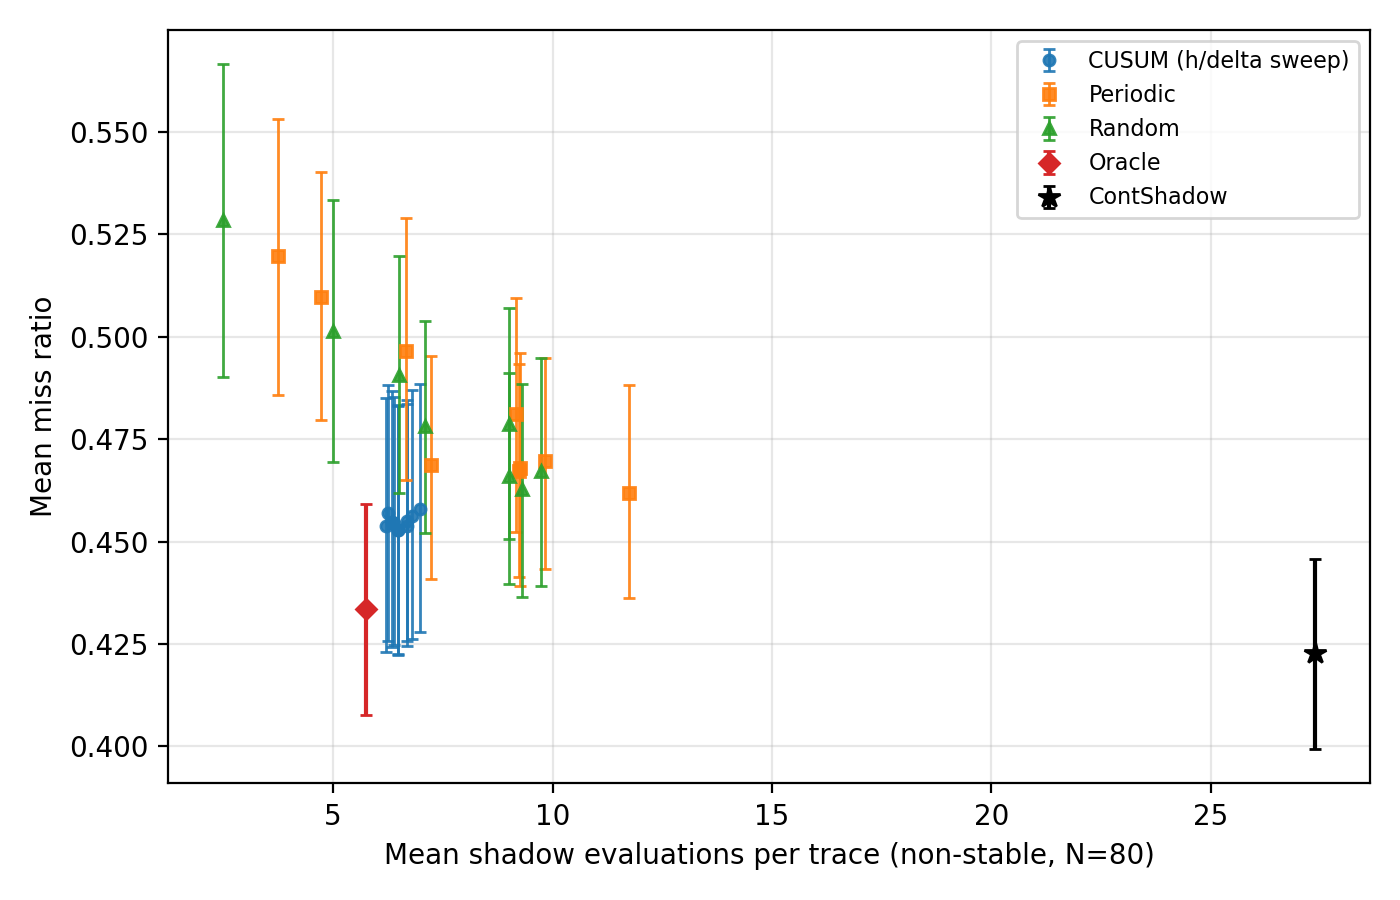
\includegraphics[width=0.85\columnwidth]{fig_phase2_frontier.png}
\caption{Post hoc Phase 2 budget-matched trigger frontier on 80 non-stable
seed-5001 traces. CUSUM dominates periodic/random at similar budgets, but
Oracle and ContShadow expose the remaining accuracy ceiling.}
\label{fig:phase2-frontier}
\end{figure}


\section{S5. Additional tables}

\begin{table}[!t]
\caption{Table S.VII. Detection with shifted phase boundaries. Each cell is \emph{detected / spurious} confirmations within a 30,000-reference absolute window after a recorded boundary; true boundaries per scenario: 100, 100, 100, 80 (zero for stable). Offsets 333 and 1501 are not multiples of the controller epoch size ($W{=}2000$). Generated by \texttt{generate\_offset\_table.py} from raw detection CSVs.}
\label{tab:offset}
\scriptsize
\setlength{\tabcolsep}{2.5pt}
\begin{tabular}{@{}lrrrrrrr@{}}
\toprule
Scenario & 0 & 250 & 333 & 500 & 1,000 & 1,370 & 1,501 \\
\multicolumn{8}{@{}l@{}}{\emph{Phase offset (references)}} \\
\midrule
Abrupt & 97/16 & 97/16 & 96/16 & 96/16 & 96/16 & 97/16 & 97/16 \\
Gradual & 24/109 & 17/114 & 17/115 & 17/113 & 24/112 & 26/112 & 19/112 \\
Recurring & 96/14 & 96/14 & 96/14 & 96/14 & 96/14 & 96/14 & 96/14 \\
Composite & 61/30 & 64/27 & 65/26 & 65/28 & 63/31 & 62/31 & 64/29 \\
\midrule
All non-stable & 278/169 & 274/171 & 274/171 & 274/171 & 279/173 & 281/173 & 276/171 \\
Stable & 0/23 & 0/23 & 0/23 & 0/23 & 0/23 & 0/23 & 0/23 \\
\bottomrule
\end{tabular}
\end{table}

\begin{table}[!t]
\caption{Table S.VIII. Mean Miss Ratio on Non-Stable Traces at $C = 500$}
\label{tab:capacity}
\footnotesize
\setlength{\tabcolsep}{7pt}
\begin{tabular}{@{}lc@{}}
\toprule
Method & Miss ratio \\
\midrule
LRU & 0.693 \\
2Q & 0.654 \\
S3-FIFO & 0.590 \\
ContShadow & 0.555 \\
DA & 0.580 \\
OPT & 0.434 \\
\bottomrule
\end{tabular}
\end{table}

\subsection*{S6. Literature Review Detail Moved from the Main Paper}
\subsection{Adaptive and Learning-Based Replacement}

3L-Cache [15] reduces the cost of learned eviction by moving learning and
inference off the critical path, evaluated on 4,855 CDN, key-value and block
traces, but its overhead remains above LRU. LPR [16] uses re-access feedback to
switch among policies at runtime, for example from LRU to MRU, with a
heuristic rather than statistical switching signal. EACLOCK [17] adapts a
CLOCK-style policy from hit-rate feedback for skewed and shifting workloads.
Clock2Q+ [18] targets correlated metadata references in VMware vSAN and reports
up to 28.5\% lower miss ratio than S3-FIFO on metadata traces. S4-FIFO [19]
learns configuration parameters for a FIFO-family heuristic rather than every
eviction, and, like 3L-Cache, separates a fast data path from slower control
logic.

\subsection{Drift Detection}

PUDD [20] detects drift from prediction uncertainty but needs a predictive
model. A label-free statistical-process-control detector [21] stresses power
and false-positive control but is evaluated by simulation of model-monitoring
scenarios. Dynamic threshold determination [22] adapts alarm thresholds after
each alarm, at the cost of maintaining parallel candidate models temporarily.
A transformer--autoencoder hybrid [23] and an HTM-plus-SPRT framework [24]
offer richer temporal modelling but impose training or univariate-data
assumptions. ADWIN-U [25] adapts adaptive windowing to unsupervised settings.
None is evaluated on page-reference streams or at memory-management rates.

\subsection{GPU, Multi-Tier and Benchmark Studies}

MSched [26] predicts the next task's working set from kernel launch arguments
to migrate GPU memory proactively, which relies on predictability that CPU page
streams lack. gpu\_ext [27] makes GPU-driver policies replaceable eBPF
programs, an architectural mechanism for safe policy updates. The LLM
prefix-cache study [28] finds LRU surprisingly competitive, cautioning against
assuming that sophisticated policies always win. A stale-tolerant cache
benchmark [29] finds that the ranking is workload-dependent across four
synthetic patterns, with ARC highest on average. Finally, Acme [34] is the closest precedent for statistical policy
switching: it simulates the alternative caching mode through shadow entries and
switches when a one-tailed $t$-test at the 0.05 level favours it, reporting
execution time within 16\% of the optimal mode in the worst case and 4\% on
average on TPC-H workloads.

Two further lines of prior art are directly relevant but were absent from the
original 15-study review. Set dueling, introduced for dynamic insertion
policies (DIP/DRRIP) by Qureshi \emph{et al.} [37], dedicates sampler sets to
two candidate insertion policies and lets the one with fewer sampler misses
control the whole cache at very low storage cost; it is the standard
low-overhead way to choose between replacement behaviours. In deployed
operating systems, the multi-generation LRU (MGLRU) reclaim path [38] groups
pages by access recency into generations and ages them incrementally, replacing
the single active/inactive list. Both are sampled or hierarchical ways of
adapting recency treatment, and both are therefore natural comparators for a
drift-gated controller. These descriptions are direct observations from the
cited sources. That the mechanisms would transfer to drift-gated page
replacement is \emph{inferred}: none of the cited evaluations measures shadow
evaluation cost, policy-state migration and post-switch warm-up together on
page-reference streams. Section~VII and the Appendix add principle-level
versions of them; the main tables predate this addition and do not include
them.


\subsection*{S6.1 Research-Gap Argument}
The reviewed work establishes that adaptive replacement is well studied
[1]--[5], [8]--[12]; that learning-based policies can respond online to
access patterns [15]--[19]; that statistical drift detection offers explicit
change evidence [6], [7], [20]--[25]; and that cache-mode selection has used
shadow evaluation and significance testing [34]. Four gaps follow.

Gap~1: detectors on reference streams. Generic drift detectors are rarely
evaluated on page-reference feature streams at memory-management sampling
rates and overhead budgets. Gap~2: statistical gating versus heuristic
adaptation. Adaptive page-replacement studies such as LPR [16] already respond
to changing patterns, but no reviewed study compares explicit statistical
change confirmation against such heuristics in a controlled experiment.
Gap~3: transition costs. The costs of detector execution, shadow simulation,
policy-state preparation and post-switch warm-up are not consistently reported
together with miss ratio and detection delay. Gap~4: comparability. Studies use
different workloads, metrics and system contexts, so their results cannot be
compared as though from a shared benchmark. Gaps~2--4 are direct observations
about the reviewed set. Gap~1 is inferred from the stated scopes of the cited
detectors; it is not a claim that no such evaluation exists outside this set.

Table~S.II (supplementary material) compares the reviewed approaches with
the controller as actually implemented in this study.



These gaps are empirical. The question is whether statistically confirmed
changes in compact page-reference summaries, combined with on-demand candidate
evaluation and explicit switching-cost safeguards, give a favourable trade-off
against fixed policies and existing adaptive methods. Each component of the
proposed controller has precedent (ADWIN [7], miniature simulation [13],
SHARDS [14], statistical cache-mode selection [34]); the claim examined here
concerns their integration for page-replacement policy selection and the
measured consequences. The review cannot establish that no related
implementation exists outside the selected literature, and the proposal is not
presented as the first statistical cache-adaptation system.


\subsection*{S7. Workloads, Baselines and Protocol Detail}
\begin{table}[!t]
\caption{Workload Definitions}
\label{tab:workloads}
\footnotesize
\begin{tabular}{@{}p{0.24\columnwidth}p{0.70\columnwidth}@{}}
\toprule
Component & Definition \\
\midrule
LOOP & Cyclic scan over 1,200 pages (larger than $C$). \\
ZIPF & Zipf(0.9) over 8,000 pages, randomly permuted page ids. \\
HOTSCAN & 70\% uniform over 600 hot pages, 30\% sequential scan over 20,000 pages. \\
WINDOW & Uniform over a 700-page window sliding one page per 40 references. \\
UNIFORM & Uniform random over 4,000 pages. \\
Stable & One primitive, 300,000 refs (6 traces each). \\
Abrupt & Six phases of 100,000 refs; no immediate repetition of a type. \\
Gradual & As abrupt, with linear mixture ramps of 40,000 refs at boundaries. \\
Recurring & Two primitives alternating, $6 \times 80{,}000$ refs. \\
Composite & Five kernel models in random order, $5 \times 100{,}000$ refs. \\
\bottomrule
\end{tabular}
\end{table}

Table~VI reports eleven non-proposed baselines (eight fixed and three
adaptive), while Table~VII pairs DA against ten of them because MRU is omitted
from the paired tests; the counts of eleven and ten refer to different tables,
not to different sets of results.

The two count-aging periods reported in Tables~IV and~V apply to different
counters, and both are intended. Table~IV describes the LFU-A policy itself:
its frequency counts are halved every $4C$ references (4,000 at
$C = 1{,}000$), and the same rule governs the LFU-A candidate inside shadow
evaluation, scaled to the capacity in use (every $4C_s = 800$ references at
$C_s = 200$). Table~V's ``Count aging'' row instead describes the controller's
own fast-path aged count (Section~V-C), which is halved every 50 epochs, i.e.\
every 100,000 references; that counter is not part of LFU-A and is used,
together with the last-access time, only to place pages when a switch migrates
state.

Re-implementations of published
algorithms follow the cited descriptions but are not the authors' code; the
LPR-style baseline re-implements the principle of [16] (re-access ``regret''
feedback with probationary LRU/MRU switching), not its code, and may differ
from the original in important ways. CAR, LIRS, CLOCK-Pro [36], CACHEUS and a
3L-style policy are included in the released simulator and raw CSVs but are not
reported in the main tables; S4-FIFO, EACLOCK and Clock2Q+ were not implemented.
The ContShadow variant is our Acme-style control: it runs the same shadow
evaluation and switching rule every ten epochs without a drift gate.

\begin{table}[!t]
\caption{Methods Compared}
\label{tab:methods}
\footnotesize
\begin{tabular}{@{}p{0.16\columnwidth}p{0.78\columnwidth}@{}}
\toprule
Group & Methods \\
\midrule
Fixed & LRU, FIFO, CLOCK, LFU-A (counts halved every $4C$ references; the rule scales with the capacity in use), MRU, 2Q ($K_{\mathrm{in}} = C/4$, $K_{\mathrm{out}} = C/2$), ARC [1], S3-FIFO [5] (10\% small queue, ghost = main size). \\
Adaptive & LeCaR [11] (re-implementation); LPR-style (principle of [16]); ContShadow (shadow evaluation every 10 epochs, no drift gate). \\
Proposed & DA: drift-gated controller (Section~V-C). \\
Ablations & DA-noPurge (A0 migration), DA-noS2 (no KS confirmation), DA-noShadow (random pick), DA-noCost (no cost margin), DA-noDwell. \\
Reference & OPT: offline Belady optimum [32]. \\
\bottomrule
\end{tabular}
\end{table}


\subsection*{S7.1 Frozen Controller Parameters}
\begin{table}[!t]
\caption{Controller Parameters Fixed After Training}
\label{tab:params}
\footnotesize
\begin{tabular}{@{}p{0.42\columnwidth}p{0.52\columnwidth}@{}}
\toprule
Parameter & Value \\
\midrule
Capacity $C$; epoch $W$ & 1,000 frames; 2,000 references \\
Sampling rate $p$ & 0.2 (hash-based, spatial) \\
CUSUM $\delta$, $h$; baseline $B$ & 0.5, 5; 8 epochs ($\sigma_0 \ge 0.02$) \\
KS level $\alpha$; window & $10^{-3}$; last 3 epochs, $\ge$ 100 samples \\
Evaluation delay; cooldown & 10 epochs; 4 epochs \\
Shadow capacity; warm-up; blocks & $\mathrm{round}(pC) = 200$; 40\%; 4 \\
LCB $z$; horizon $H$; margin $K$ & 1.28; 50,000 refs; $K = 0$ in frozen run (design default $0.1C = 100$) \\
Dwell $D$; hysteresis window & 10 epochs; 30 epochs \\
Migration purge age & 20,000 references \\
Count aging & halved every 50 epochs \\
\bottomrule
\end{tabular}
\end{table}


\subsection*{S7.2 Cluster-Sampling Sensitivity Note}
\emph{Sensitivity only.} As a coarse check we also resample the
four scenario clusters; with four clusters this yields only $\binom{7}{4}=35$
distinct resamples. It gives DA--S3-FIFO $-0.0154$ [$-0.0294$, $-0.0048$],
excluding zero where the primary trace-level paired interval does not. Because
35 resamples cannot support a reliable interval, this result is reported only
as a sensitivity note and is never used as the headline uncertainty statement.


\subsection*{S8.1 Scenario-Level Replacement Quality}
By scenario the controller was close to ContShadow on abrupt (0.370 versus
0.365) and recurring (0.398 versus 0.384) traces, but clearly behind it on
gradual drift (0.439 versus 0.401) and composite (0.604 versus 0.541). The
gap on gradual drift matters because the paper's premise is detection of slow
change; the CUSUM trigger usually reacts only after the mixture has moved.


\subsection*{S8.2 Paired Differences, DA Minus Baseline}
\begin{table}[!t]
\caption{Paired Differences, DA Minus Baseline (Non-Stable, $N = 80$)}
\label{tab:paired}
\footnotesize
\setlength{\tabcolsep}{4.5pt}
\begin{tabular}{@{}lcccc@{}}
\toprule
Baseline & Mean diff. [95\% CI] & W/L/T & Holm $p$ \\
\midrule
LRU & $-0.1171$ [$-0.140$, $-0.094$] & 75/5/0 & $<0.001$ \\
FIFO & $-0.1472$ [$-0.171$, $-0.124$] & 75/5/0 & $<0.001$ \\
CLOCK & $-0.1065$ [$-0.130$, $-0.084$] & 75/5/0 & $<0.001$ \\
LFU-A & $-0.0933$ [$-0.116$, $-0.071$] & 74/6/0 & $<0.001$ \\
2Q & $-0.0691$ [$-0.090$, $-0.048$] & 71/9/0 & $<0.001$ \\
ARC & $-0.0758$ [$-0.099$, $-0.053$] & 71/9/0 & $<0.001$ \\
S3-FIFO & $-0.0154$ [$-0.035$, $+0.004$] & 42/38/0 & 0.090 \\
LeCaR & $-0.0980$ [$-0.121$, $-0.076$] & 72/8/0 & $<0.001$ \\
LPR-style & $-0.0800$ [$-0.098$, $-0.061$] & 70/10/0 & $<0.001$ \\
ContShadow & $+0.0301$ [$+0.016$, $+0.045$] & 15/54/11 & $<0.001$ \\
\bottomrule
\end{tabular}
\end{table}


\subsection*{S8.3 Post Hoc Repair on Synthetic Traces}
\emph{Post hoc design correction (synthetic traces).} The capacity-sampling
repair described in Section~V-I was re-selected on the training
traces only using the same 48-configuration grid and selection rule with
\texttt{--cs-cap-f 1.0}. It selected the same configuration
($n_{\mathrm{cand}}{=}5$, $K{=}0$, delay 10). Evaluated once on the 80
non-stable and 30 stable held-out test traces, the repaired controller
produced miss ratios, switch counts, and shadow-evaluation counts identical to
the original controller. This post hoc correction therefore did
not change the synthetic-trace outcome.


\subsection*{S8.4 Ablation, Activation Counts and Figure}
Table~\ref{tab:ablation} removes one component at a time. The dominant result
is that shadow evaluation is essential: replacing it by a random choice raised
the non-stable miss ratio from 0.453 to 0.619, worse than LRU. The remaining
variants scored 0.453--0.456, a small range that must be interpreted with the
activation counts below. Additive diagnostic logging of the frozen main-study
run (byte-identical outputs to the released simulator) records how often each
component actually acted across the 110 traces. The recency filter acted at
47 of the 213 switches, dropping 39,405 stale pages from the migrated resident
set. The KS stage was active on all 643 alarms and rejected 173 of them, after
which 570 shadow evaluations were performed; its small ablation effect is not
because it never fired. The cost margin never acted ($K = 0$, so no cost-margin
decision was made) and the dwell rule never blocked a switch (zero blocks):
under the frozen configuration these two components were \emph{inactive}, and
the ablation cannot estimate their benefit from these runs. Counting an
inactive component as ``showing no benefit'' would conflate absence of
activation with absence of effect. Table~\ref{tab:ablation} also includes
S3-FIFO as a static reference: at 0.468 miss ratio and 28.5 ns/reference it is
cheaper than DA but less accurate, so neither policy Pareto-dominates the
other on these generated traces. ContShadow reached 0.423 with 27.39 shadow
evaluations per trace against 6.47 for DA, a 76.4\% reduction, but it was
more accurate: the saving in shadow work was \emph{not} at equal miss ratio on
the generated traces. On the real-program traces below the two methods do tie
on miss ratio.

\begin{table}[!t]
\caption{Ablation on the Fresh Test Traces (Non-Stable Mean)}
\label{tab:ablation}
\footnotesize
\setlength{\tabcolsep}{5pt}
\begin{tabular}{@{}lcccc@{}}
\toprule
Variant & Miss ratio & Switches & Shadow evals & ns/ref \\
\midrule
DA & 0.453 & 2.36 & 6.47 & 67.4 \\
DA-noPurge & 0.453 & 2.36 & 6.47 & 68.5 \\
DA-noS2 & 0.456 & 2.27 & 6.76 & 67.9 \\
DA-noShadow & 0.619 & 5.05 & 0.00 & 77.3 \\
DA-noCost & 0.453 & 2.36 & 6.47 & 66.9 \\
DA-noDwell & 0.453 & 2.36 & 6.47 & 67.9 \\
S3-FIFO (static reference) & 0.468 & 0.00 & 0.00 & 28.5 \\
ContShadow & 0.423 & 3.15 & 27.39 & 133.4 \\
\bottomrule
\end{tabular}
\end{table}

\begin{figure}[!t]
\centering
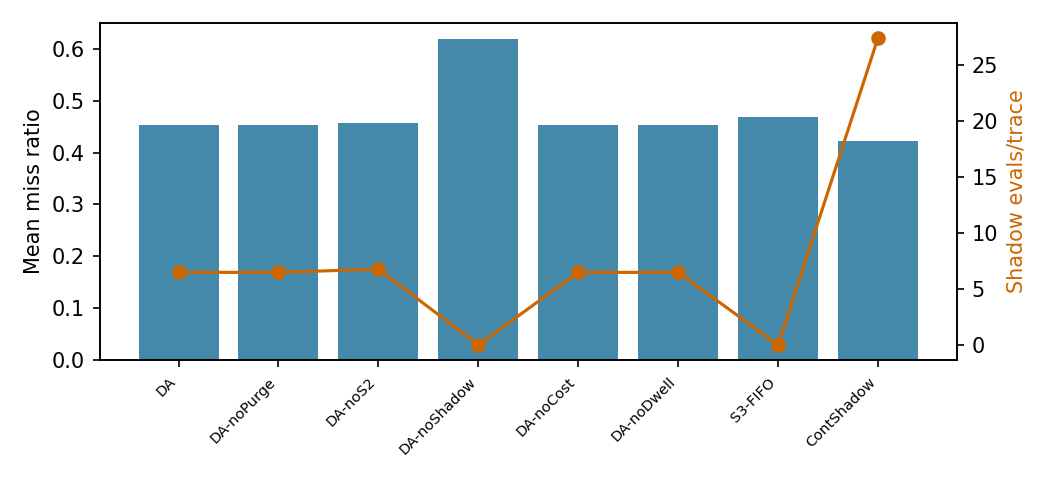
\includegraphics[width=0.85\columnwidth]{fig6_ablation.png}
\caption{Ablation: non-stable miss ratio and shadow evaluations per trace.}
\label{fig:ablation}
\end{figure}


\subsection*{S8.5 Detection and Boundary-Offset Detail}
The CUSUM trigger detected 278 of 380 phase boundaries (73.2\%) over the four
non-stable scenarios, with a median confirmation delay of 2,000 references:
97/100 abrupt, 24/100 gradual, 96/100 recurring and 61/80 composite. Detection
is therefore strong for abrupt and recurring changes and weak for gradual
ones. This value is conditional on the boundary alignment described below.
Boundaries in the generator coincide with epoch boundaries, which favours
detection, so neither figure should be read as a real-system detection rate.
Of the 169 spurious confirmations outside the 30,000-reference boundary
windows, 16 occurred on abrupt, 109 on gradual, 14 on recurring and 30 on
composite traces: the gradual scenario, already the hardest to detect,
produced about two-thirds of all false alarms. On the 30 stable traces there
were 23 spurious confirmations, but only one after reference 100,000. Of the
23, 17 occurred before reference 50,000, five between 50,000 and 100,000, and
the remaining one at reference 160,000; the 100,000-reference exclusion thus
removes 22 of the 23, and the residual late confirmation is a genuine
long-horizon false alarm rather than an initial transient. The controller
switched 2.36 times per non-stable trace against 3.15 for ContShadow.

\emph{Detection with shifted phase boundaries.} The generator's change points
fall on controller-epoch boundaries, which favours detection. The released
simulator's \texttt{--phase-offset} option prepends a given number of
references from the first phase before the first boundary and shifts all
recorded boundaries by that amount; with offset zero the main detection output
is reproduced exactly. Table~S.VII (supplementary material) reports seven offsets generated
directly from raw detection CSVs by \texttt{generate\_offset\_table.py},
including 333 and 1501 references, which are not multiples of the controller
epoch size ($W{=}2000$). Detection is counted within a 30,000-reference
absolute window after each recorded boundary. Across offsets the trigger
detected between 274 and 281 of 380 boundaries (72.1\%--73.9\%) and produced
between 169 and 173 spurious confirmations; offset 0 was neither best nor
worst. Stable traces produced 23 spurious confirmations at every offset.

Gradual drift remains weakly detected: 24 of 100 gradual boundaries were
detected at offset 0 (17--26 across offsets), while gradual traces produced 109
spurious confirmations at offset 0. This means the paper's drift-gating premise
is supported only for sharper regime changes in this study; slowly moving
workloads can cross the miss-ratio threshold without a reliable CUSUM
confirmation.



The raw CSV rows, the exact simulator commands and the diagnostic event-log
schema are collected in the supplementary material accompanying this paper.


\subsection*{S8.6 Cost--Quality Figure and Interpretation}
\begin{figure}[!t]
\centering
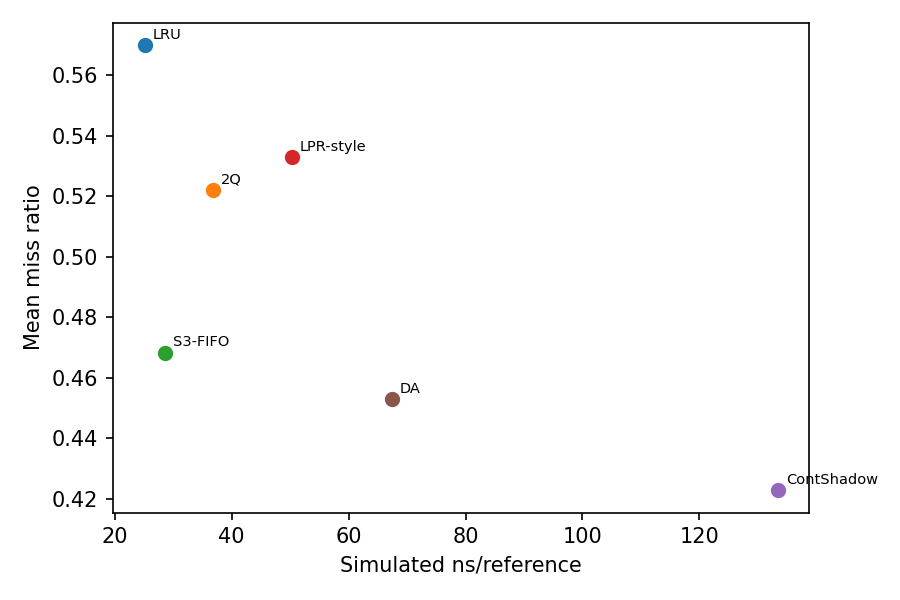
\includegraphics[width=0.85\columnwidth]{fig7_cost.png}
\caption{Miss ratio against simulated time per reference (indicative,
single-threaded simulator); S3-FIFO is included as a static comparator.}
\label{fig:cost}
\end{figure}


\subsection*{S9. Post Hoc Trigger, Detector-Parameter and Rankability Detail}
\emph{Trigger variants (synthetic, post hoc).} The released simulator was
modified to add \texttt{--trigger cusum|periodic|random|oracle},
\texttt{--trigger-period}, \texttt{--trigger-rand}, \texttt{--trigger-seed},
and \texttt{--delta}; default CUSUM DA output was verified byte-identical to
the released main-study DA rows (110 rows, 0 mismatches, detection
identical). On the same 80 non-stable seed-5001 test traces, DA-oracle
(mean miss 0.4335, 2.19 switches, 5.74 shadow evals) was better than DA
(0.4529, 2.36, 6.47), while DA-periodic-p40 (0.4687, 2.52, 7.22) and
DA-random-r04 (0.4906, 2.60, 6.50) were worse. Paired DA-minus-other
differences (bootstrap 10,000, seed 0; Wilcoxon/Holm) were: DA-oracle
$+0.0194$ [$+0.0061,+0.0347$], W/L/T 8/22/50, Holm $0.0177$; DA-periodic-p40
$-0.0158$ [$-0.0297,-0.0008$], W/L/T 36/26/18, Holm $0.0177$; DA-random-r04
$-0.0377$ [$-0.0585,-0.0163$], W/L/T 47/19/14, Holm $0.0004$; DA-ContShadow
$+0.0301$ [$+0.0167,+0.0454$], W/L/T 15/54/11, Holm $2.51{\times}10^{-5}$.
The oracle variant uses synthetic ground-truth boundaries and is not a
deployable trigger.

\emph{FIU trigger check (post hoc).} Using the same six FIU test traces and
base args as the FIU rankability runs (default seed 5001, default $C=1000$),
DA-oracle had mean miss 0.712698, 6 switches, 6 shadow evals, and 0 confirms;
DA-periodic-p40 had 0.713068, 11, 40, 35 confirms; DA-random-r04 had
0.709742, 10, 36, 35 confirms. The corresponding baseline at $C=1000, p=0.2$
was 0.706285 mean miss, 10 switches, 46 shadow evals
(\texttt{rankability\_real/fiu\_C1000\_p0.2.csv}). The oracle produced no
confirmations because these FIU trace files expose no ground-truth bounds in
the trace format; this result is not evidence of oracle benefit on FIU.

\emph{Parameter sensitivity (synthetic, post hoc).} One-at-a-time sweeps from
the default DA configuration (seed 5001, 80 non-stable + 30 stable traces)
showed: $W\in\{1000,2000,4000\}$ gave miss 0.461442, 0.452888, 0.500050;
$\delta\in\{0.1,0.3,0.5,0.7,1.0\}$ gave 0.457896, 0.455087, 0.452888,
0.454430, 0.453678; $h\in\{2,3,5,7,10\}$ gave 0.456338, 0.453806, 0.452888,
0.454700, 0.456900; $p\in\{0.05,0.1,0.2,0.4\}$ gave 0.480957, 0.469601,
0.452888, 0.447180. These measurements describe local sensitivity around the
frozen configuration and do not replace the train-only selection protocol.

\emph{Capacity/sampling rankability (post hoc).} The synthetic sweep
($C\in\{500,1000,2000,4000\}$, $p\in\{0.05,0.1,0.2,0.4\}$) showed mean miss
decreasing with larger $C$ (e.g., $C=500,p=0.2$ 0.580196; $C=4000,p=0.2$
0.180884) with nonzero switches/evals in all tested cells
(\texttt{rankability\_real/synth\_sweep.csv}). The FIU sweep
($C\in\{500,1000,2000,5000,10000,20000\}$, same $p$ grid) showed
$C=20000$ gives mean miss 0.668337 with 0 switches for all $p$, while smaller
$C$ values show switches and miss variation
(\texttt{rankability\_real/fiu\_sweep.csv}). These real measurements
characterize rankability/capacity behavior but do not provide a new external
validation win.


\subsection*{S10. Public Block-Trace Setup and Conversion}
The generated traces have controlled change points, which favours the
controller. As an external check the released simulator was run on six FIU
web/block traces from the CMU PDL cacheDatasets collection [39], obtained from
the repository's \texttt{fiu/} directory. The released converter
\texttt{convert\_public\_traces.py} reads the packed 24-byte request records
(timestamp, object id, object size, next-access time) and maps object ids to
dense identifiers in first-touch order. The first 1,000,000 requests of each
trace were used, except \texttt{madmax}, which contains 918,010 requests; the
single-thread page-id array requires \texttt{--np 1048576}. The replay
capacity $C = 20{,}000$ was selected on a \emph{separate} PDL trace,
\texttt{fiu\_webusers-030409-033109.oracleGeneral.zst}, which is not one of the
six evaluated traces. The recorded post hoc grid was $C \in \{1000, 5000, 10000,
15000, 20000, 25000, 50000\}$ with seed 0, methods LRU and S3-FIFO (DA was also
run for the record). The rule selected the smallest $C$ at which both miss
ratios were at least 0.01 and LRU exceeded S3-FIFO by at least 0.10: at
$C = 10{,}000$ the miss ratios were 0.74182/0.73317 (gap 0.00865), and at
$C = 20{,}000$ they were 0.73590/0.52726 (gap 0.20864), so $C = 20{,}000$ was
selected. The raw pilot CSVs, manifest and exact commands are in
\texttt{phase10\_capacity\_pilot/}. The earlier \texttt{webresearch}-only pilot
(\texttt{public\_pilot\_C*.csv}) is retained for provenance but is not the
selection source. The frozen main-study controller configuration and the
default seed 5001 apply to the six evaluated traces. The exact replay commands
are given in the supplementary material.


\subsection*{S10.1 FIU Diagnostics, Re-selection and Repair}
\emph{Per-trace diagnostics and a capacity--sampling fault.} To check for a
sampling or implementation fault, each public trace was re-run with an
additive diagnostic build of the released simulator that logs the CUSUM
statistic and per-candidate shadow margins without changing control flow
(identical miss ratios, switch counts and shadow-evaluation counts; byte-identical
detection CSV). The CUSUM alarm threshold $h = 5$ was crossed on every trace:
maximum $S^+$ ranged from 7.95 to 20.30 and maximum $S^-$ from 6.08 to 33.30,
so the trigger fired normally. Yet every shadow evaluation returned identical
miss counts for all five candidates --- for example, 1,120 misses for LRU,
LFU-A, 2Q, MRU and S3-FIFO on \texttt{webresearch} at reference 16,000 --- giving
zero per-candidate margins and a tie-break to candidate 0 (LRU) in every
initial selection and every later decision. S3-FIFO is a candidate in DA
(candidate id 4), so its 0.577 stand-alone miss ratio was simply never visible
to the controller. The cause is an interaction between capacity and sampling:
the shadow cache holds $C_s = p\,C = 0.2 \times 20{,}000 = 4{,}000$ pages, more
than the roughly 1,100--1,800 distinct pages in each sampled evaluation window,
so all candidates incur only compulsory misses and cannot be ranked. At the
synthetic-study capacity $C = 1{,}000$ ($C_s = 200$) the same trace gives
differentiated counts (1,141 / 1,137 / 1,139 / 1,885 / 1,135 for candidates
0--4 at reference 16,000), S3-FIFO wins the initial selection and DA makes one
switch. The no-switch result on the public traces is therefore a
capacity--sampling fault in this configuration, not evidence that candidate
policies are equivalent on real workloads. Per-trace maxima and margins are in
the supplementary material.

\emph{Parameter re-selection on training prefixes.} Each public trace was split
into a 500,000-reference training prefix and a held-out suffix (418,010
references for \texttt{madmax}; 500,000 for the others), and the 48-configuration
selection grid was re-run on the six prefixes. All 48 configurations produced
the same training mean miss ratio (0.68027) and zero switches, because the
capacity--sampling fault makes the controller parameters inert at $C = 20{,}000$;
the tie-break selected $n_{\mathrm{cand}} = 4$, $K = 0$, evaluation delay 2. On
the held-out suffixes the re-selected configuration and the frozen one
($n_{\mathrm{cand}} = 5$, $K = 0$, delay 10) both achieved mean miss 0.66834 with
zero switches; the re-selected run was cheaper per reference (67.6 versus 85.0
ns) only because it evaluated four candidates instead of five. These runs are
reported as a failed external validation, not as a tuned result.

\emph{Post hoc design correction.} A post hoc repair caps shadow capacity at
$C_s=\min(\mathrm{round}(pC),\mathrm{round}(f D_w))$, where $D_w$ is the
number of distinct sampled page IDs in the evaluation window and $f=1.0$ is
fixed a priori. With $f=1.0$ this is an identity cap: it changes $C_s$ only
when $D_w < pC$, but when all candidates fit in the sampled distinct-page
set they still tie on compulsory misses. It therefore cannot create
rankability where $pC$ already exceeds $D_w$; a real fix must reduce $C_s$
below $D_w$ or increase $D_w$ relative to $C_s$. The repair is implemented
behind \texttt{--cs-cap-f} (default 0, disabled) and leaves the original
behaviour byte-identical. Re-running the 48-configuration selection on the
same training prefixes with \texttt{--cs-cap-f 1.0} produced the same training
mean miss ratio (0.68027) and zero switches for every configuration; the
tie-break selected the same configuration. On the held-out suffixes, the
repaired controller achieved the same mean miss ratio as the original
(0.66834) with zero switches. The post hoc repair therefore did not change
the public-trace outcome.


\subsection*{S11. Cost Model Derivation and Envelope Detail}
The measured trade-off in Section~V-F is a 0.030 miss-ratio penalty for DA
against a 66.0 ns/reference time saving and 20.9 fewer shadow evaluations per
trace. Whether that is a good trade depends on what a miss costs. Let $c_m$ be
the cost of one miss (page fault plus service) and $c_e$ the cost of one shadow
evaluation, both in nanoseconds. With the same fast path for both methods, the
total time per trace is
\begin{equation}
T = N t_0 + N m c_m + E c_e,
\label{eq:cost}
\end{equation}
where $N$ is the trace length, $m$ the miss ratio, $E$ the number of shadow
evaluations, and $t_0$ the per-reference cost excluding shadows. DA beats
ContShadow in total time iff
\begin{equation}
(m_{\mathrm{DA}} - m_{\mathrm{CS}})\,c_m
+ (E_{\mathrm{DA}} - E_{\mathrm{CS}})\,c_e/N < 0,
\label{eq:breakeven}
\end{equation}
i.e.\ $c_e > R c_m$ with
$R = N(m_{\mathrm{DA}} - m_{\mathrm{CS}})/(E_{\mathrm{CS}} - E_{\mathrm{DA}})$.
Using the measured means ($m_{\mathrm{DA}}=0.453$, $m_{\mathrm{CS}}=0.423$,
$E_{\mathrm{DA}}=6.47$, $E_{\mathrm{CS}}=27.39$, and $N=545{,}000$ for the
average non-stable trace), \texttt{cost\_model.py} recomputes $R = 783.28$,
i.e.\ $R \approx 783$: one shadow evaluation must cost more than about 783
misses for DA to beat ContShadow. A 10,000-replicate trace-level bootstrap
(\texttt{bootstrap\_cost\_model.py}, seed 20261123) gives a 95\% percentile CI
of $[426, 1187]$ for $R$. Equivalently, the direct measured-time comparison
$T \approx t + m c_m$ gives a DA--ContShadow crossover of
$(133.4-67.4)/(0.453-0.423) = 2196\,\mathrm{ns} \approx 2.2\,\mu$s per miss
(\texttt{cost\_model.csv}), with a 95\% bootstrap CI of
$[1.44, 4.06]\,\mu$s (\texttt{cost\_model\_bootstrap.csv}). Both figures depend
on the unoptimized simulator timings; the ratio is more robust than the
absolute scale, and the intervals are wide because the 80-trace sample has a
heavy tail. These are DA-versus-ContShadow comparisons; the total-time table
gives the full total-time comparison over four policies and
the total-time figure plots it. S3-FIFO is already a candidate in DA's shadow
set (candidate id 4 in \texttt{mkCand}); DA pays the gating and evaluation
overhead even when it selects S3-FIFO.

\textbf{Total-time envelope.}
Using the measured means (CLOCK 0.559 miss ratio at 8.90\,ns/reference,
S3-FIFO 0.468 at 28.54\,ns, ContShadow 0.423 at 133.36\,ns, DA 0.453 at
67.36\,ns), the lower envelope is CLOCK for $c_m<0.216\,\mu$s, S3-FIFO for
$0.216<c_m<2.305\,\mu$s and ContShadow for $c_m>2.305\,\mu$s. DA is never on
the envelope: its smallest excess over the best policy is
3.27\,ns/reference at $c_m\approx2.305\,\mu$s. At the measured minor-fault
cost (1.98--2.06\,$\mu$s) S3-FIFO is cheapest and DA is about 5\,ns/reference
above it. DA beats ContShadow only below 2.196\,$\mu$s, but S3-FIFO stays
cheaper than DA until 2.517\,$\mu$s. A 10,000-replicate trace-level bootstrap
(seed 20261124, \texttt{phase5/bootstrap\_total\_time.py}) gives 95\% intervals
of $[0.171,0.274]\,\mu$s (CLOCK/S3-FIFO), $[1.660,3.678]\,\mu$s
(S3-FIFO/ContShadow), $[1.449,4.105]\,\mu$s (DA/ContShadow) and
$[1.086,22.05]\,\mu$s (DA/S3-FIFO; unstable because the miss-ratio difference
is small); the minimum-gap interval is $[-28.6,40.2]$\,ns, so the ranking at
the crossing is not statistically resolved. The point estimates nevertheless
show no miss cost at which DA is cheapest.

To check the implied evaluation cost directly, a timing-only build of the
released simulator (no diagnostic logging) measured 570 shadow evaluations on
the same traces at a mean of $2.46$\,ms and a median of $2.33$\,ms each. The
cost model's time decomposition implies $1.72$\,ms per evaluation, so the
direct measurement is about $1.4\times$ higher; both are simulator-side
numbers from an unoptimized single-threaded build and should be read as an
order-of-magnitude check, not a kernel latency. Because the directly measured
evaluation cost exceeds the implied one, the DA--ContShadow crossover would
occur at a somewhat lower miss cost than the $2.2\,\mu$s point estimate, which
further weakens the case for gating under minor-fault-dominated costs.


\subsection*{S11.1 Calibration and Analytical Async Variant}
The 2.2\,$\mu$s point is a user-space minor-fault calibration
(\texttt{prototype\_fault\_latency.cpp}), not a kernel page-fault latency.
On the evaluation machine, a first-touch minor fault on a 4\,KiB anonymous page
costs 1.98\,$\mu$s and a refault after \texttt{MADV\_DONTNEED} costs
2.06\,$\mu$s (medians over seven 128\,MiB runs; a resident access costs
16\,ns). The other $c_m$ rows are illustrative parameter ranges, not measured
on this system; they show how the DA--ContShadow crossover moves with miss
penalty. At this calibration S3-FIFO is cheapest and DA is close to
ContShadow; for larger miss penalties ContShadow's lower miss ratio dominates.
Across all miss costs DA is above the lower envelope of CLOCK, S3-FIFO and
ContShadow (the total-time table). An analytical async-shadow variant
(\texttt{phase5/async\_model.csv}, assumption: evaluation fully off the
request path, same miss ratios, background CPU proportional to evaluations)
removes evaluation latency from the critical path but leaves the miss-ratio
difference unchanged; it therefore does not convert DA into an accuracy win
over ContShadow. Absolute times are from an unoptimized single-threaded
simulator; the DA--ContShadow ratio is the more robust quantity.


\subsection*{S8.7 Capacity Sensitivity at C = 500}
Table~S.VIII (supplementary material) repeats the primary comparison at $C = 500$. The controller scored
0.580 against LRU 0.693 and S3-FIFO 0.590, but was again behind ContShadow
(0.555). The $C = 2{,}000$ and sampling-rate runs are present in the released
raw CSVs; full-shadow ranking agreement was not measured, so we make no claim
from it.


\subsection*{S8.8 Design Lessons}
The design lessons are narrow. First, shadow
evaluation is the component that matters: without it the controller is worse
than LRU. Second, the CUSUM trigger with sampled shadow evaluation reduced
shadow work by 76\% relative to continuous evaluation under the frozen cost-margin
rule ($K = 0$), but here it cost 0.030 in mean miss ratio; gating is a
cost-saving mechanism, not an accuracy advantage in the generated study. Third,
the KS stage had a small miss-ratio effect, while the cost margin and dwell
rule were inactive in the frozen run ($K = 0$, zero dwell blocks) and the
recency filter acted at 47 of 213 switches. KS was enabled in the frozen run,
while the margin was $K = 0$; the
effective mechanism was therefore a CUSUM trigger with sampled shadow
evaluation, not a validated two-stage gate. Fourth, on the fifteen-program
appendix the gated controller and continuous evaluation tie on miss ratio, but
DA costs 2.4 times S3-FIFO and does not beat it. Fifth, the cost model shows
that DA beats ContShadow only when a miss costs less than about 2.2 $\mu$s,
but the full total-time envelope puts CLOCK below 0.216\,$\mu$s, S3-FIFO
between 0.216 and 2.305\,$\mu$s and ContShadow above 2.305\,$\mu$s, with DA
never cheapest on the measured means. We therefore report where gating saves
shadow work, and do not claim that DA is best in these measurements or superior
to strong replacement policies.


\subsection*{S12. Threats to Validity Detail}
\emph{Construct validity.} The traces are generated: five synthetic access
primitives and five kernel-level access models, not traces recorded from
running systems. Generated phases have clean boundaries aligned with the controller's epochs,
which favours detection delay, and workload types such as loops larger than
memory are overrepresented relative to their frequency in practice, which
favours policies such as MRU and regret-driven LRU/MRU switching. The reported
73.2\% detection rate (278/380) and roughly 2,000-reference
median delay are therefore conditional on this alignment and overstate what
would be expected under asynchronous drift in a real system. Miss ratio is also partly determined by the active policy, so the
CUSUM monitor can mistake a policy-induced change for workload change; the KS confirmation was designed
to address this, but in the frozen run it had only a small miss-ratio effect
(0.456 without KS vs.\ 0.453 with KS) despite being active on all 643 alarms.

\emph{Internal validity.} The controller configuration was selected by a sweep
on training traces before the fresh test set was touched. We mitigated the
resulting selection freedom by freezing all parameters and evaluating the test
traces once; nevertheless, the configuration was chosen to minimize training
miss ratio, and a reader should treat it as one degree of freedom.
Re-implementations of ARC, S3-FIFO, 2Q, LeCaR and the LPR-style
heuristic may differ from the original implementations, and baselines were not
tuned per workload, which can favour or penalize them. The simulator was
sanity-checked against known behaviour but not against reference
implementations. Seeds were fixed and the shadow simulator's sampling is
deterministic.

\emph{External validity.} A single-threaded trace-driven simulator omits
concurrency, memory pressure from multiple processes, reclaim interactions,
writeback, I/O queueing and NUMA effects. Cost figures come from an
unoptimized simulator on a shared virtual machine and should be read as
relative magnitudes. Results at one nominal capacity (with sensitivity at one other) and one trace
length may not transfer to other scales. Findings are
limited to the evaluated workload families.

\emph{Statistical conclusion validity.} The switching rule applies a normal
quantile ($z = 1.28$) to only four autocorrelated shadow blocks; a
$t$-quantile with three degrees of freedom is about 1.64, so the nominal 90\%
bound is optimistic. A post hoc seed-5001 robustness run with
$t_{0.90,3}$ gave DA miss 0.4586 [0.4282,0.4888] vs default 0.4529
[0.4224,0.4834]. KS $p$-values on dependent, tied reuse times are not calibrated error rates,
so the confirmation stage provides a heuristic gate rather than formal error
control; its ablation showed a small miss-ratio effect (0.456 vs.\ 0.453), and
the effective mechanism is better described as a CUSUM trigger with sampled
shadow evaluation. KS was enabled in the frozen run, the margin was $K = 0$, and no
validated two-stage statistical gate is claimed. Traces within a scenario share a generator,
so the effective number of independent workloads is smaller than 80, and the
stated $p$-values and intervals describe variability over generated traces,
not over real workloads. Wilcoxon tests with ten corrected comparisons have
limited power for differences of about 0.01 in mean miss ratio. No cost budget or agreement threshold was specified before the study. Several secondary results (for
for example the small KS ablation difference) are small or non-significant
differences and should not be read as evidence of no effect.


\subsection*{S12.1 Limitations and Scope Detail}
This paper evaluates one controller design in a single, released simulator,
and it does not establish that the controller outperforms the best existing
replacement algorithms. In the reproducible main study the controller (0.453)
was 20.5\% below LRU (0.570) and better than S3-FIFO (0.468) on the mean, but
the S3-FIFO difference was not significant (adjusted $p = 0.09$), and
continuous shadow evaluation was significantly more accurate (0.423). The
controller cost 2.7 times LRU and 2.4 times S3-FIFO. The 76\% reduction in
shadow evaluations therefore came with a 0.030 loss in miss ratio in the main
study, not at equal miss ratio; only the real-program appendix shows a tie. We
make no claim of competitive cost or quality.

The present study is reproducible from the released package, but the main
results remain a trace-driven simulation. Real in-kernel fault-path durations
were later measured in a nine-boot QEMU guest (Section~S14), but no reclaim
function was reached and no in-kernel DA policy was built. CAR,
LIRS, CLOCK-Pro, CACHEUS, a 3L-style policy, an MGLRU-style policy and
set-dueling DIP are present in the released simulator and CSVs but are not
reported in the main tables; S4-FIFO, EACLOCK and Clock2Q+ were not implemented.
We do not claim the MGLRU-style implementation as a faithful baseline: a
page-level trace replay has no kernel aging or reclaim-pressure signal, so it
reduces to generation-indexed LRU rather than Linux MGLRU [38]. The frozen
controller used the five-candidate set including S3-FIFO; adding S3-FIFO
improved the miss ratio but did not make DA clearly better than the static
policy.

The KS confirmation had a small miss-ratio effect in the main study (0.456
without KS vs.\ 0.453 with KS) and was active on all 643 alarms. The cost
margin and dwell rule were inactive in the frozen configuration ($K = 0$, zero
dwell blocks), so their ablations do not estimate their benefit. The recency
filter acted at 47 of 213 switches without changing the mean miss ratio. The
effective mechanism was a CUSUM trigger with sampled shadow evaluation, not a
validated two-stage statistical gate. The evidence
is generated, with phase boundaries aligned to epochs and loop-heavy workloads
overrepresented; both choices favour detection and MRU-like heuristics. The
real-program traces come from fifteen instrumented kernels, six of which have
miss ratios below 0.02 at $C = 1000$; fifteen program-level clusters give
limited power and the mean is dominated by five high-miss kernels where DA and
S3-FIFO are nearly tied. A faithful kernel MGLRU baseline is not available:
the reported MGLRU-style policy is a page-level abstraction. The QEMU guest
observes the kernel's own MGLRU and measures fault-path duration only; no
reclaim latency was measured and the cost model uses a user-space minor-fault
calibration. The public traces are storage block/cache traces, not
paging traces, and only a prefix of each was replayed. The four-cluster
bootstrap of the synthetic main study has only 35 distinct resamples and is
reported as a coarse sensitivity check only. The literature review is
narrative, not systematic, and its limitations in Table~I are partly inferred.

Post hoc measurements (Section~V-J) and recorded post hoc follow-ups
(Section~V-K) characterize trigger variants, rankability,
detector alternatives, stronger baselines, and cost uncertainty. The oracle
trigger uses synthetic ground-truth boundaries and is not deployable; the FIU
oracle produced no confirmations because FIU trace files expose no
ground-truth bounds. PH/ADWIN/SIEVE/W-TinyLFU/LHD are independent simplified
implementations in the released simulator with documented assumptions; they
are not authors' reference implementations. Available real-trace follow-ups
used 6 FIU public split traces (500k-request prepared splits), 15-program
traces, and three original FIU traces downloaded from [39] at deterministic
1/5/10\% WSS capacities.

The main remaining gaps are external validity and system implementation.
Bounded 1M-reference prefixes of the other six PDL families (MSR Cambridge,
Alibaba, Tencent, CloudPhysics, Twitter and MetaKV) were downloaded and run in
Phase~6 (Section~S14); the [39] repository, FIU trace filename, README and
site-wide non-commercial copyright notice were verified, but no
dataset-specific licence file was found, so use is reported as non-commercial
research with citation rather than as use under a dataset licence. A real
asynchronous shadow-evaluation prototype was built and measured in
Phase~7. A kernel-faithful MGLRU baseline and an in-kernel DA replacement
prototype were not built; the Phase~8 guest observed the kernel's existing
MGLRU and measured fault-path latency, but no reclaim event was reached. The
cost calibration remains a user-space minor-fault microbenchmark. These
limitations bound the claims to the evaluated simulator, traces, guest
observation and calibration.


\subsection*{S13. Exploratory Real-Program Evidence Moved from the Appendix}
\emph{Uncertainty note.} The trace-level interval is the primary uncertainty
statement throughout. As a sensitivity note only, the four-cluster bootstrap
on the synthetic traces has $\binom{7}{4} = 35$ distinct cluster resamples and
gives DA--S3-FIFO $-0.0154$ [$-0.0294$, $-0.0048$], excluding zero where the
primary trace-level paired interval does not. With only 35 resamples this is a
coarse check, not reliable evidence either way.

\emph{Real programs and whole-program holdout.} We recorded page traces by
instrumenting fifteen real programs: an index tree, a chained hash join, a CSR
breadth-first search, an in-place quicksort of 20-byte records, a column-major
Jacobi stencil, sparse-matrix value gathers, a binary heap with random
decrease-key, a histogram scatter over a 16 MB key array, a random walk over a
CSR adjacency array, an open-addressing hash table, a column-major
matrix-vector product over a 32 MiB matrix, pointer chasing through a 64 MiB
linked list, random-window string search over a 16 MiB text, union-find with
path compression over four million elements, and binary search over a 32 MiB
sorted key array. Four seeds were recorded per program (300,000 references
each; $C = 1000$, 100,000 warm-up). To remove seed-level leakage, we held out
\emph{whole programs}: for each of fifteen folds,
all tunable baselines and DA were tuned on the other fourteen programs and
evaluated once on the four traces of the omitted program. We also added
principle-level implementations of CAR, LIRS, CLOCK-Pro, CACHEUS, a 3L-style
policy, set-dueling DIP [37] and an MGLRU-style policy [38]; assumptions are
marked in the released source. The MGLRU-style policy is a page-level
abstraction of Linux MGLRU, not a kernel-faithful baseline: trace replay has no
kernel aging or reclaim-pressure signal.



The whole-program holdout means (Table~S.III in the supplementary material) are summarized here: The comparisons
below are exploratory; percentile intervals, Wilcoxon p-values, and Holm
adjustment are generated from the fifteen whole-program folds by the released
\texttt{appendix\_intervals.py} (bootstrap seed 7, 10,000 resamples) and are
fragile with fifteen clusters and many ties. With per-fold tuning and
whole-program holdout DA scored 0.3304, 6.7\% below LRU (0.3540). A post hoc
capacity-sampling repair ($f{=}1.0$, fixed a priori; \texttt{--cs-cap-f 1.0})
evaluated with the same whole-program holdout protocol produced identical mean
miss ratios to the original controller (DA 0.3304, S3-FIFO 0.3291, LRU 0.3540).



After Holm correction across these ten comparisons no difference remains
significant (smallest adjusted $p=0.096$ for 2Q). DA was not better than
S3-FIFO on average, so these fifteen-program results do not establish
superiority over the best static policy. Six of the fifteen kernels have miss ratios below 0.02 at this
capacity (hash join, breadth-first search, sort, stencil, radix scatter and
string search), and the mean is dominated by five high-miss kernels (sparse
gathers 0.72, random walk 0.83, hash table 0.71, linked list 0.94 and
union-find 0.73), where DA and S3-FIFO are nearly tied. In this independent
simulator, measured on the same 60 traces with the default frozen
configuration, DA cost 59.5 ns/reference against 27.5 for LRU and 24.7 for
S3-FIFO (2.2 and 2.4 times); the main-study 2.7-times figure differs because
the implementations and workloads differ, and on both DA is slower than
S3-FIFO. These are instrumented kernels, not production traces; the appendix
does not establish superiority or measure kernel latency. Source, seeds,
configurations, raw CSV output and analysis scripts, including
\texttt{appendix\_intervals.py}, are released in the accompanying reproduction
package.


\section{S14. Additional Measured Checks (Phases 6--8)}
The six 1M-reference CMU PDL prefixes were replayed at 18 family$\times$capacity
points with the frozen controller configuration. The full method means are
reproduced below; the abbreviated table in the main paper retains the five
methods discussed there.
\begin{table}[t]
\caption{Phase 6: means over 18 PDL family$\times$capacity points (1M-reference prefixes)}
\label{tab:pdl_all}
\centering\footnotesize
\begin{tabular}{@{}lcccc@{}}
\toprule
Method & Mean miss & Switches/trace & Shadow evals/trace & ns/ref \\
\midrule
ARC & 0.4796 & 0.00 & 0.00 & 56.4 \\
CLOCK & 0.4973 & 0.00 & 0.00 & 9.5 \\
ContShadow & 0.4739 & 1.06 & 13.11 & 147.5 \\
DA & 0.4742 & 0.83 & 2.67 & 94.4 \\
LHD & 0.7278 & 0.00 & 0.00 & 125.3 \\
LRU & 0.4987 & 0.00 & 0.00 & 41.0 \\
S3-FIFO & 0.4683 & 0.00 & 0.00 & 43.4 \\
SIEVE & 0.4879 & 0.00 & 0.00 & 21.1 \\
W-TinyLFU & 0.4857 & 0.00 & 0.00 & 157.3 \\
\bottomrule
\end{tabular}
\end{table}

The paired DA-minus-baseline table in
\texttt{reproduction/phase6\_pdl/paired\_da\_minus\_baseline.csv} gives a
DA--S3-FIFO paired difference of $+0.0059$ (bootstrap CI $+0.0026$ to
$+0.0093$), Wilcoxon $p=0.0092$ and Holm $p=0.0192$; 11 of 18 points favour
S3-FIFO, four tie and three favour DA. This is a negative result for DA
relative to S3-FIFO on these prefixes.

The real user-space asynchronous shadow worker was run three times on the 80
non-stable seed-5001 traces. The measured mean miss ratios were 0.5611, 0.5676
and 0.5599; paired async-minus-sync differences were $+0.1082$, $+0.1147$ and
$+0.1070$, with win/tie/loss counts 12/0/68, 9/0/71 and 8/0/72. The worker
timing summary (\texttt{phase7\_async/timing\_summary.csv}) records 240
non-stable timing rows, 15,066 stale decisions, 1,192 applied results, 0
dropped results and 0 superseded results. Async execution is therefore clearly
worse than the synchronous controller in these measurements.

A Linux 6.6.1 guest kernel was then built from source under an unprivileged
user path and booted nine times under QEMU: three fresh boots each for fixed
LRU (\texttt{lru\_gen/enabled=0x0000}), fixed MGLRU (\texttt{0x0007}) and a
user-space CUSUM controller coupled to the same sysfs knob. The build used
\texttt{gcc-15 -std=gnu11}, locally built bison 3.8.2 and elfutils 0.191
libelf; the tarball SHA256, config options, compiler versions and controller
constants (10\,ms interval, $h=5$, $\delta=0.5$, 10-epoch delay) are recorded in
\texttt{phase8\_kernel/manifest.csv}. The six failed build/boot attempts
(missing headers, C23 keyword conflicts, link order, absent dynamic loader,
absent \texttt{/dev/null}, a filter file outside the mounted results directory
and missing \texttt{uname}) were recorded in \texttt{PROTOCOL.md} and discarded
before any measurement; no number from them is used here.

Function-graph tracing was restricted to the five recorded fault and
reclaim functions present in the guest. Parsing the raw traces yielded 191,370
per-function duration samples in 18 condition$\times$repetition$\times$function
groups, all reproduced in Table~\ref{tab:kernel_ftrace}. Only
\texttt{handle\_mm\_fault} and \texttt{do\_wp\_page} produced samples. The
\texttt{handle\_mm\_fault} median/p95 durations ranged from 641/1532\,ns
(fixed MGLRU, repetition 1) to 761/1593\,ns (fixed LRU, repetition 1); no
reclaim function was reached. The main-paper table lists the matching per-run
vmstat deltas: every one of the nine runs has
131,138 minor faults, zero major faults, zero \texttt{workingset\_refault\_anon}
events and zero \texttt{pgscan\_anon}/\texttt{pgsteal\_anon} deltas. The
controller wrote no toggles in any of its three runs because its signal never
became positive. The captured cgroup \texttt{memory.max}, \texttt{memory.swap.max}
and \texttt{memory.peak} files were empty, so the guest did not demonstrate
memory pressure and these runs provide no reclaim-latency measurement. This is
a real in-kernel fault-path timing observation under an MGLRU-enabled guest,
not an in-kernel DA replacement policy or a kernel-faithful MGLRU comparison.

\begin{table}[t]
\caption{Phase 8: per-function ftrace durations from the guest kernel (all conditions)}
\label{tab:kernel_ftrace}
\centering\footnotesize
\setlength{\tabcolsep}{2pt}
\begin{tabular}{@{}lccccc@{}}
\toprule
Condition & Rep. & Function & Samples & Median ns & p95 ns \\
\midrule
coupled & 1 & do\_wp\_page & 47 & 1423.0 & 4024.8 \\
coupled & 1 & handle\_mm\_fault & 21289 & 731.0 & 1673.0 \\
coupled & 2 & do\_wp\_page & 48 & 2119.0 & 4988.9 \\
coupled & 2 & handle\_mm\_fault & 21467 & 741.0 & 1693.0 \\
coupled & 3 & do\_wp\_page & 32 & 1663.0 & 7649.4 \\
coupled & 3 & handle\_mm\_fault & 21198 & 701.0 & 1583.0 \\
fixed\_lru & 1 & do\_wp\_page & 11 & 1493.0 & 2133.5 \\
fixed\_lru & 1 & handle\_mm\_fault & 21206 & 761.0 & 1593.0 \\
fixed\_lru & 2 & do\_wp\_page & 11 & 2304.0 & 3546.0 \\
fixed\_lru & 2 & handle\_mm\_fault & 21201 & 671.0 & 1522.0 \\
fixed\_lru & 3 & do\_wp\_page & 11 & 1462.0 & 4303.5 \\
fixed\_lru & 3 & handle\_mm\_fault & 21203 & 752.0 & 1643.9 \\
fixed\_mglru & 1 & do\_wp\_page & 11 & 1994.0 & 4574.0 \\
fixed\_mglru & 1 & handle\_mm\_fault & 21207 & 641.0 & 1532.0 \\
fixed\_mglru & 2 & do\_wp\_page & 11 & 1253.0 & 1778.5 \\
fixed\_mglru & 2 & handle\_mm\_fault & 21204 & 711.5 & 1573.0 \\
fixed\_mglru & 3 & do\_wp\_page & 10 & 1583.0 & 2049.5 \\
fixed\_mglru & 3 & handle\_mm\_fault & 21203 & 741.0 & 1643.0 \\
\bottomrule
\end{tabular}
\end{table}


\end{document}
